\documentclass{article}
\usepackage{comparison}

\usepackage{expl3,xparse}

\ExplSyntaxOn

\NewDocumentCommand \ProgramName { m } {
  \textsl{#1}
}

\NewDocumentCommand \MicrosoftWord { } {
  Microsoft~\ProgramName{Word}
}

\NewDocumentCommand \MyEmail { } {
  \href{mailto:seallred@smcm.edu}{\texttt{seallred@smcm.edu}}
}

\NewDocumentCommand \wysiwyg { } {
  \textit{what-you-see-is-what-you-get}
}

\NewDocumentCommand \WYSIWYG { } {
  \textit{What-You-See-Is-What-You-Get}
}

\NewDocumentCommand \UseCanned { m } {
  \input{../../canned/#1}
}

\ExplSyntaxOff

%%% Local Variables: 
%%% mode: latex
%%% TeX-master: nil
%%% End: 

\usepackage{booktabs,array,pdfpages,hyperref}

\newcommand{\twcomp}[2]{%
  \vspace{2ex}
  \par\noindent
  \Compare{\TeX}{#1}
          {\MicrosoftWord}{#2}
  \vspace{2ex}
  \par\noindent
}

\usepackage{fontspec,xltxtra}
\setmainfont[Ligatures=TeX]{Hoefler Text}

\title{The Beauty of \TeX}
\author{Sean Allred}

\usepackage{mwe,kantlipsum}
\begin{document}
\maketitle

\begin{abstract}
As opposed to \MicrosoftWord,
  \TeX\ is run on an input file and
  doesn't need to produce the final copy
  several times a second.
This means that \TeX\ can spend
  the necessary time needed
  to make your document
  look absolutely \emph{gorgeous},
  not to mention exceptionally readable.
(After all, \TeX\ was written to typeset the author's own books;
 his publisher's work (especially for mathematics) was not up to his standards.)
This short article hopes
  to expose some of the finer details
  of \TeX's workmanship.
\end{abstract}
\vfil
\tableofcontents
\newpage

\section{Kerning}
\label{sec:kerning}

\NewTerm{Kerning} is that space which separates the letters of a word.
It isn't particularly a property of the text that many people explicitly \emph{notice},
  but it is one that can make a word look \emph{bad} or \emph{good}.
Of course, those who know about kerning are \emph{cursed},\footnote{%
  \url{http://www.xkcd.com/1015} CC--BY--NC Randall Munroe.}
  but it is good to be able to spot the work of a professional,
  and kerning is one example of a professional concern.

\begin{center}
  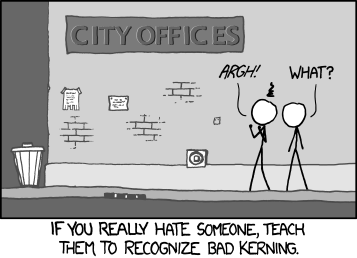
\includegraphics[width=.5\linewidth]{xkcd-kerning}
\end{center}

\noindent
There are certain letters in the Latin alphabet that
  require special spacing when used together.
Most letters are mostly box-shaped (`h', `s', \dots),
  but there are several that have space
  throughout most of the glyph (`Y', `T', `L', \dots)
  or can otherwise look awkward when combined recklessly.
Thus, most typesetters in the days of hand-printing
  made special stamps for these combinations
  that had spacing that looked right.

Today, computers---not typesetters---control most of our document needs.
Computers do not follow these practices by default,
  and products like \MicrosoftWord\ simply do not have the capability.
Sometimes, this is barely noticeable (but still ugly to the trained eye),
  while other times the blunder is obvious and simply obtrusive.
See \autoref{tab:compare} for a visual comparison.



\section{Ligatures}
\label{sec:ligatures}

\NewTerm{Ligatures} are another such special treatment of letters.
When combined, some letters can `clash' with each other in rather ugly ways.
While viewed up close the `smushed' glyphs may seem a little strange,
  their appearance in text often goes unnoticed.
Free from the microdistraction of clashing letters,
  the reader is able to, well, read!
See \autoref{tab:compare} for a visual comparison.

\section{Small Caps}
\label{sec:small-caps}

\section{Justification}
\label{sec:justification}


\appendix

\begin{table}
  \centering
{
  \def\resize{\LARGE}
  \def\notex{\addfontfeature{Ligatures=NoCommon,Kerning=Off}}
  \begin{tabular}{ c c }
    \toprule
    \TeX & \MicrosoftWord \\
    \midrule
    \resize Table & \resize\notex T\kern.5ptable \\
    \resize SALT & \resize\notex SAL\kern.6ptT \\
    \resize AVAST & \resize\notex A\kern.3ptV\kern.3ptAST \\
    \resize\slshape AVAST & \resize\notex\slshape A\kern.3ptV\kern.3ptAST \\
    \resize `L' & \resize\notex `L\kern1pt' \\
    \midrule
    \resize efficient firefly & \resize\notex ef\kern1ptf\kern1pticient f\kern.2ptiref\kern1.5ptly \\
    \resize fiery fjord & \resize\notex f\kern.8ptiery f\kern.8ptjord \\
    \midrule
    \resize \textsc{Small Caps} & \resize\notex S{\normalsize MALL} C{\normalsize APS} \\
    \midrule
    \multicolumn{2}{p{.7\linewidth}}{For a comparison of justification, please refer to the last page of this article for an example and statistical analysis written by Roel Zinkstok for Zink~Typography.}\\
    \bottomrule
  \end{tabular}
}
  \caption{A comparison of \TeX\ and other word processing solutions
    (such as \MicrosoftWord) in regards to
    kerning, ligatures, and small capitals}
  \label{tab:compare}
\end{table}


\lipsum\noindent
\includegraphics[width=\linewidth]{example-image-a}

\cleardoublepage
\includepdf{comparison}
\end{document}

%%% Local Variables: 
%%% mode: latex
%%% TeX-master: t
%%% TeX-engine: xetex 
%%% End: 
